\documentclass[a4paper,11pt]{article}

\usepackage[slovene]{babel}
\usepackage[utf8]{inputenc}

\usepackage{listings}
\usepackage{babelbib}
\usepackage{url}

\usepackage{graphicx}
\usepackage{float}
\graphicspath{ {images/} }
\usepackage[usenames, dvipsnames]{color}

\usepackage{multicol,caption}

\newenvironment{Figure}
  {\par\medskip\noindent\minipage{\linewidth}}
  {\endminipage\par\medskip}


\usepackage{multicol}
\setlength{\columnsep}{1cm}

\usepackage{underscore}
\renewcommand{\lstlistingname}{Primer}% Listing -> Primer

\usepackage{amsmath}
\usepackage{bm}

\usepackage{array}
\usepackage{tabu}

\lstset{
numbers=left, 
numberstyle=\small, 
numbersep=8pt, 
frame = single, 
language=Python, 
framexleftmargin=15pt}

\setlength{\parindent}{0pt}
%BORDERS
\usepackage{geometry}
 \geometry{
 a4paper,
 total={170mm,257mm},
 left=30mm,
 right=25mm,
 top=30mm,
 bottom=30mm
 }

\begin{document}

\huge { Priporočanje športnega treninga na podlagi prejšnjih aktivnosti\\\\} 
\normalsize
[Summary]
\\

\begin{multicols}{2}

\section{Uvod}
Veliko ljudi se dandanes ukvarja z najrazličnejšimi športi, nekateri profesionalno, z namenom, da dosežejo čim boljše rezultate in osvojijo medalije na tekmovanjih, drugi pa se s športom ukvarjajo povsem rekreacijsko. Skoraj vsi športniki pa se borijo s samim sabo in želijo doseči nek cilj.\\
Kot glavni faktor, ki pripomore k izboljšavm lahko štejemo kritike, mnenja in predloge, ki jih dobimo od trenerjev oz. akterja, ki spremlja našo športno aktivnost. Trenutna tehnologija omogoča bogat nabor podatkov, ki jih lahko dobimo v času treningov in tekem. Veliko atletov in trenerjev se strinja, da do ti podatki neprecenljivega pomena\cite{Liebermann}. Velika večina ljudi ima danes ob sebi pametne telefone, nekateri celo pametne ure in razne športne ure, ki omogočajo zbiranje podatkov o aktivnosti osebe, natančnost podatkov pa je odvisna od tipa posamezne naprave in proizvajalca čipa\cite{Case}.\\
Pridobljeni podatki, nam brez prave obdelave in predstavitve ne prinašajo velike vrednosti, zato bomo v  članku opisali metode, s katerimi smo podatke obdelali in iz njih pridobili uporabne informacije. Naša naloga je bila preizkusiti različne metode strojnega učenja, ki bi trenerjem in rekreativnim športnikom pomagale pri priporočanju čim bolj optimalnega treninga.\\
V nadaljevanju članka, je so navedena in opisana povezana dela in že odstoječe aplikacije, ki obstajo na tem področju. Opisan je postopek priprave podatkov in uporabljene metode strojnega učenja. V drugem delu čanka pa je predstavljen eksperiment in rezultati našega dela.


\section{Povezana dela}
[Tukaj povezana dela]

\section{Priprava podatkov}
[Parser in podatki itd....]

\section{Metode strojnega učenja}
Razvitih je bilo že kar nekaj metod strojnega učenja, v našem primeru je bila izbira metode strojnega učenja prepuščena posamezniku, saj smo si želeli čim večjo raznolikost. Izbrali smo si \textit{odločitveno drevo}, \textit{nevronske mreže}, \textit{metodo podpornih vektorjev (SVM)}, na koncu pa smo poskusili še z ansambelsko metodo.

\subsection{Odločitveno drevo}


\subsection{Nevronske mreže}


\subsection{Metoda podpornih vektorjev}
Metodo podpornih  vektorjev (\textit{angl. Support vector machine}) je prvič leta 1995 predstavil V. Vapnik\cite{Vapnik}, ki jo je opisal kot metodo nazdorovanega strojnega učenja za binarne klasifikacijske probleme. SVM je v primerjavi z nevronskimi mrežami precej enostavnejša metoda, ki ne zagotavlja ravno optimalnih rezultatov, omogoča pa nam da hitro dosežemo sprejemljive rezultate\cite{Hsu}.\\
SVM je uporabljen na mnogih področjih, kot je klasifikacija slik, razpoznava ročno napisanih črk, v raziskovalne namene v biologiji in drugih znanstvenih podtočjih, najbolje pa se obnese pri kategorizaciji besedila\cite{Wiki_svm}.\\
\subsubsection{Prednosti SVM}
Razlogi za izbiro metode SVM so: \cite{SciDev}:
\begin{enumerate}
\item{deluje v večdimenzionalnem prostoru,}
\item{efektiven tudi v primeru, jo je število atributov večje, kot število primerkov,}
\item{prostorko učinkovit,}
\item{podpira različne funkcije jedra}
\end{enumerate}

\subsubsection{Slabosti SVM}
Kot vsaka metoda, ima tudi ta slabosti \cite{SciDev}:
\begin{enumerate}
\item{slabša učinkovitost v primeru da je število atributov veliko večje od števila primerkov,}
\item{SVM-ji direktno ne določajo verjetnosti, zato je ta izračunana s pomočjo \textit{five-fold cross-validation}}
\end{enumerate}


\section{Predstavitev eksperimenta}
Eksperiment, smo izvedli s pomočjo lastnega ogrodja zasnovanega na programskem jeziku \textit{Python} in z uporabo knjižnice \textit{scikit-learn}, ki že ima implementirane vse metode strojnega učenja, ki smo jih pri delu potrebovali, za vizualizacijo rezultatov, pa smo izdelali vizualizacijsko orodje. 


\subsubsection{Nabor podatkov}

\subsubsection{[Tukaj pride še nekaj podnaslovov s področja eksperimenta]}
[Predlagam da si pogledata strukturo, ki je uporabljena pri JT in se ji poskušata pribljižati]

\subsubsection{Eksperiment}

\subsubsection{Vizualizacijsko orodje}
Vizualizacija podatkov je prav tako pomembna, kot obdelava, saj je potrebno rezultate predstaviti na primeren način, tako da je uporabniku prijazen. Naše vizualizacijsko orodje je povsem ločeno od ogrodja za izvajanje eksperimenta. Orodje temelji na programskem jeziku \textit{JavaScript} in na popularni knjižnici za obliko \textit{Bootstrap}.\\
Orodje kot vhod pričakuje podatke v obliki strukture \textit{JSON}, ki jih nato predstavi v obiki urnika.\\ 


\begin{Figure}
 \centering
 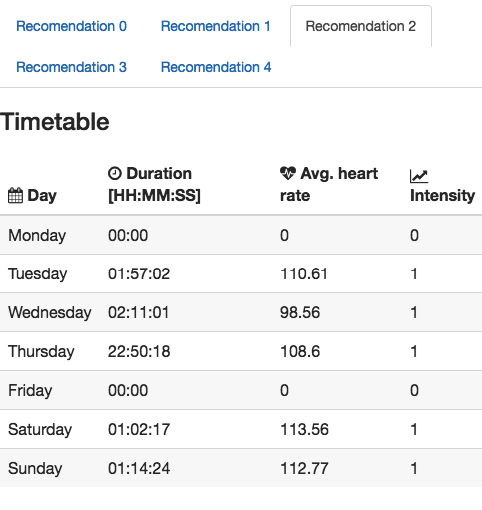
\includegraphics[width=\linewidth]{vizualization}
 \captionof{figure}{Prikaz vizualizacije}
\end{Figure}


\subsection{Rezultati}


\subsection{Zaključek}


\end{multicols}

\normalsize
\newpage

\begin{multicols}{2}


\bibliography{mybib}{}
\bibliographystyle{plain}

\end{multicols}

\end{document}